\documentclass[10pt,journal,compsoc]{IEEEtran}
\usepackage{graphicx}
\usepackage{upgreek}
\graphicspath{ {Images/} }
%\usepackage{algorithm}
\usepackage{algpseudocode}
\usepackage[linesnumbered,ruled]{algorithm2e}
\usepackage{hyperref}
\usepackage{verbatim}
\usepackage{amsmath,bm,amssymb,amsbsy, amsthm, mathtools}
\usepackage{caption}
\usepackage{graphicx,epsf, epsfig, epstopdf, epsfig, subFigure}
\usepackage{pifont}
\usepackage{hyperref}
\usepackage{colordvi}
\usepackage{soul} % to highlith sentences put \hl{}
\usepackage{array}%tabel header
\usepackage{multirow}%tabel
\usepackage{lipsum}%tabel vertical alignment
\usepackage{csquotes}
\usepackage{url}
%*********************************************************
\ifCLASSOPTIONcompsoc
  \usepackage[nocompress]{cite}
\else
  \usepackage{cite}
\fi
\ifCLASSINFOpdf
\else
\fi
\hyphenation{op-tical net-works semi-conduc-tor}
%*********************************************************
\begin{document}

\title{The Study of Weather Effects on COVID-19 }

%-------------------------------------------------------------
\author{Joshua Francisco, Micah Mercado, Xavier Mercado, Harpreet Ghag, Michael Novella, Madhuri Pyreddy
	\IEEEmembership{Matin~Pirouz }% <-this % stops a space

%	\IEEEcompsocitemizethanks{\IEEEcompsocthanksitem "Harpreet Ghag" with the Department
%		of Computer Science, California State University, Fresno .\protect\\
%		E-mail:  orange101@mail.fresnostate.edu
%		\IEEEcompsocthanksitem M. Pirouz is a faculty in the Department of Computer Science, California State University, Fresno\protect\\
%		E-mail:  mpirouz@mail.fresnostate.edu}% <-this % stops an unwanted space
	\thanks{Manuscript received April 25, 2020}}
%-------------------------------------------------------------
\markboth{Journal of \LaTeX\ Class Files,~Vol.~, No.~8, August~2019}%
{Shell \MakeLowercase{\textit{et al.}}: Bare Demo of IEEEtran.cls for Computer Society Journals}
\IEEEtitleabstractindextext{%
%#############################################################################################################################
\begin{abstract}
Given data-sets  COVID-19 mortality rate, and weather aspects such as temperature, ozone levels, and humidity when the virus was present, we present our method of analyzing weather effects with mortality rate to see if weather can have an effect on COVID-19.
\end{abstract}
%#############################################################################################################################
\begin{IEEEkeywords}
 Coronavirus, covid-19, humidity, ozone, temperature, mortality, weather
\end{IEEEkeywords}}
%#############################################################################################################################
\maketitle
\IEEEdisplaynontitleabstractindextext
\IEEEpeerreviewmaketitle
\IEEEraisesectionheading{
%#############################################################################################################################
\section{Introduction}
\label{sec:introduction}}

The current 2020 COVID-19 pandemic  (or the Coronavirus) has been affecting everyone in almost all aspects of life - school, work, and general lifestyle. One lifestyle change for everyone is the concept of social distancing which entails people staying away from each other by at least six feet. Also, quarantining oneself inside their home instead of going out has been another lifestyle change. Both methods are being used by everyone as a community effort to flatten the curve or reduce the amount of COVID-10 cases. Currently, scientists are conducting research to find a cure or vaccine for the virus. With the season shifting towards summer, news outlets have mentioned weather having an effect on COVID-19. This is similar to the case of the SARS (severe acute respiratory syndrome) outbreak and the effects of weather on this virus. \cite{Tan-2005}

	This specific area of study - weather effects and its interactions with viruses such as COVID-19, SARS, Ebola have not been heavily researched like other scientific topics. This is due to the fact that these pandemics do not occur often along with the level and capacity of technology not being readily available back then in terms of data and performance. Some studies have been done on smaller pandemic viruses like SARS and Ebola but have not given a clear and definitive conclusion as to whether or not weather has a direct effect on viruses. Although the small quantity of research (compared to other topics and fields of science), this is important as the analyses and results can provide insight and direction to determine what needs to be done or what can be expected in case of future pandemics.

	In this paper, we study multiple aspects of weather - ozone levels, humidity, and temperature to determine if they have an effect on Coronavirus, this is the main question we aim to investigate. Besides the fact that these aspects directly affect our lives, temperature has been the main focus of weather affecting viruses in other research regarding this topic. The inclusion of other aspects of weather, ozone and humidity, gives an alternate angle to this topic and possibly a different result. To measure ozone levels and humidity, we analyze the two aspects of weather over different latitudes between two specific dates. These dates we analyzed are February 6, 2020, and March 14, 2020. In February, coronavirus cases started to appear in countries such as Italy, China, and the United States. During the month of February coronavirus cases were not as prevalent. In March, the coronavirus was oficially announced as a global pandemic with an increased rate and amount in Coronavirus cases. These specific dates highlights certain days of those respective months where the rate and amount of cases show a drastic shift, which is why these dates were chosen. We relate this to COVID-19 by taking data of the Coronavirus mortality rate and analyze it with each aspect of weather we are studying - ozone, humidity, temperature.

	As we can see in most viruses, it is highly probably that COVID-19 can die off due to exposure to higher temperature rates. We can also see a possibility that areas across various latitudes, with varying ozone and humidity, have a certain range of COVID-19 mortality rate. By comparing graphs and data from COVID-19 mortality rate to weather related graphs and data, we can gain information from this relationship. We believe that there is a discernable pattern between weather and COVID-19. It seems that at latitude forty (40th parallel north), there are locations with both warmer climates and higher COVID-19 mortality rates. As the season shifts towards summer, the days become hotter, with a possibilility that COVID-19 could still remain prevalent based on our findings. News outlets and scientists mention the possibility of a second wave of COVID-19 cases coming with quarantining and social distancing still being the primary solutions and effective means to combat the amount of Coronavirus cases.

%#############################################################################################################################
% Literature Review
\section{Literature Review}
\label{literature review}

	In this section, we present various related works of weather and its multiple aspects such as ozone, humidity, and temperature to see if they have an effect on the coronavirus and other studies relating to this topic. We also provide some studies that show the similarities between Coronavirus and SARS.
	
	%2
	The article “Spread of SARS-CoV-2 Coronavirus likely to be constrained by climate” by Miguel B. Araujo and Babak Naimi is a study on using different ecological models that use weather and COVID-19 data. \cite{Araujo-2020} They say that the Coronavirus outbreaks are mainly existent in the warmer and also temperate climates will have increased possibility of a fast spread of the virus. This is related to our current topic in that we want to explore how weather can be a factor in how Coronavirus spreads throughout the world. In the article, the team behind this states "higher latitude regions of the southern hemisphere are projected to face increases in climate suitability for outbreaks of SARS-CoV-2." The point behind this comes from the research backed by the models the team has done from examining different climate zones and comparing them to the coronavirus outbreak points. \cite{Araujo-2020}

	%3
	The article "Effect of weather on COVID-19 spread in the US: A prediction model for India in 2020" by Sonal Gupta, Gourav Singh Raghuwanshi, and Arnab Chanda provides another look at the effect weather can have on the virus during this time.\cite{Gupta-2020} The time tested ranged from January 1, 2020 through April 2, 2020. The researchers in the study found that most new cases were occurring, within a ten day interval, in areas that had a humidity of 4 to 6 grams per cubic meter. \cite{Gupta-2020} The article uses that information as a way to simulate what would happen if COVID-19 spread to India. \cite{Gupta-2020} Using this information we try to solidify our reasoning to pursue this topic but on a global level.

	%4
	The article "Temperature, Humidity and Latitude Analysis to Predict Potential Spread and Seasonality for COVID-19" by Mohammad M. Sajadi, et al, is about proposing the idea that temperature and humidity play a role in the spread of the COVID-19. \cite{Sajadi-2020} Areas of low to mild humidity are at high risks of being places where the outbreak can happen. \cite{Sajadi-2020} This was found out by performing statistical modeling of where outbreaks have been most prominent, and then comparing them to the temperature, humidity, and general placement to help determine where the virus may strike next. \cite{Sajadi-2020} From the article, we understand that lower humid areas around 3-4 g/m \^ \ 3 in the north eastern places of the planet are more susceptible to the outbreaks. \cite{Sajadi-2020}

	%5
	The article "Stability of SARS-CoV-2 in different environmental conditions" by Alex W. H. Chin, et al, provides a source for looking at how COVID-19 acts under prolonged exposure to different temperatures and surfaces. \cite{Chin-2020} The findings from their article was that COVID-19 can live on smooth surfaces longer at room temperature, around 22°C. \cite{Chin-2020} From this study we can gather that COVID-19 is highly susceptible to low heat, but it also depends on the surface on which the virus resides upon. We took this information into account when trying to figure what to do from the ozone and temperature datasets. 

	%6
	The article \textit{Will Coronavirus Pandemic Diminish by Summer?} by Qasim Bukhari, et al., provides another look at modeling absolute humidity and temperature comparative to the outbreaks of COVID-19. \cite{Bukhari-2020} This article helps back the team's idea of how weather plays a role in how the virus spreads. The article goes through the same process of looking at absolute humidity and temperature and then determining if there is a correlation between that and the outbreaks of the virus. We use this article as a support for investigating this set of correlations. Written within the article's abstract, it suggests that, \ "it is extremely unlikely that the spread of 2019-nCoV would slow down in the USA or Europe, due to environmental factors \ ". \cite{Bukhari-2020} In making this comment, the article implies that temperature may not play that much of a role in the spread of the virus, but the physical contact itself.

	%7
	The article \textit{Social distancing strategies for curbing the COVID-19 epidemic} by Stephen M Kissler, et al, is about the different ways that people can implement social distancing and its impact. \cite{Kissler-2020} The article goes through different methods of social distancing factoring advocating for social distancing measures. Seasons play a role in how COVID-19 is similar to the flu, thus allowing their team to make mathematical models based off of existing information on flu data. This is relevant to our research in those areas most affected by winter or summer cold to determine which type of social distancing should be done.

	%8
	In the article, \textit{COVID-19} by Khae Hawn Kim featured in the International Neurourology Journal, Kim discusses non-medical impact on the people from this virus. \cite{Kim-2020} The author emphasizes how this virus is seen as the biggest threat to people's lives and that the pandemic is bigger than anything we have seen. This holds relevancy by showing how devastating the Coronavirus is. From our research, we hope that people will have a better idea of what to do in the future.

	%9
	 \textit{The simulations driving the world’s response to COVID-19} by David Adam, featured in the journal \ " Nature\ ", talks about the multiple ways people use algorithms to predict how COVID-19 can spread and how effective it can be for the populous \cite{Adam-2020}. This article is useful for our research in that, from their research, we are able to receive more information and prediction for our data sets. The article provides inference into how people can use prediction on social distancing and other etiologies for the virus. \cite{Adam-2020} Inference looks at the density of the population and its proportion to the virus spread.

	%10
	The article \textit{Potential Factors Influencing Repeated SARS Outbreaks in China} published in the International Journal of Environmental Research and Public Health displays the many influences of SARS and COVID-19. \cite{Sun-2020} Potential factors include animal carriers and human interactions. \cite{Sun-2020} This article is useful to our research in that it takes into account that human movement is a more prominent factor to play in the spread of the virus. This seems more likely to happen for the virus than weather.

	%11
	In the article, \textit{Role of temperature and humidity in the modulation of the doubling time of COVID-19 cases} by Barbara Oliveiros, et al, provides a model for predicting how temperature can influence COVID-19. \cite{Oliveiros-2020} They predicted that there's a slight uptick in cases during the summer months from previous cases and their relation in China. \cite{Oliveiros-2020} Problems arise in that researchers only used the data relevant to China. \cite{Oliveiros-2020} This is overlooked as research and the prediction done is looked at stretched across the world for our research.

	%12
	In the journal Science of the Total Environment, an article titled \textit{Effects of temperature variation and humidity on the death of COVID-19 in Wuhan, China} uses weather data to help simulate where large outbreaks are occuring. \cite{Ma-2020} This article is mainly used as a guide on what data to look for in our research. Also, this article supports our hypothesis that humidity and ozone are affecting the spread of COVID-19.

	%13
	The article \textit{Temperature, Population and Longitudinal Analysis to Predict Potential Spread for COVID-19} explains researchers who studied temperature uses and population within the world to determine where outbreaks of COVID-19 would occur. \cite{Dangi-2020} This article serves as a backbone to help build our hypothesis. It is also stated that populations in high densities will likely have an outbreak. \cite{Dangi-2020}

%#############################################################################################################################
% Methods Begin
\section{Methods}\label{sec:methods}

	After taking into account that weather does have an effect on the SARS virus and the many similarities that SARS has compared to Coronavirus, we delve deeper into this idea. First we wanted to find reliable open data online, and went through the process of researching and finding suitable datasets to back our claim. We found a wide variety of sources but we primarily stuck to using kaggle as some of the data we found proved to be a reliable source of information with their data being collected by reputable sources. The data sets we collected were for countries that are affected by the Coronavirus. One of the data sets we used includes weather data sets with weather aspects such as ozone, humidity and mortality rate data sets.

	In our descriptive analysis, we found a strong correlation between latitude and the date March 14, 2020. We also found another strong correlation between latitude and the date February 6, 2020. Ozone levels in countries affected with the Coronavirus are consistent. Later shown in our visuals, if we look towards our “Ozone Measure at Different Latitudes/Longitudes” graph, there are high ozone levels in China and Europe. This correlates with the mortality rate graph previously mentioned and shows some relation in high ozone to high mortality rate. However, it proves that the ozone levels in countries did not fluctuate, thereby making it impossible for the countries’ ozone levels to be affected by Coronavirus.

	We were able to find a very strong correlation between the latitude and the date March 14, 2020. We also found another strong correlation between latitude and February 6, 2020. Here we see that humidity levels in these countries affected by the Coronavirus fluctuate. Taking this into account, it it highly possible that the Coronavirus can be affected by humidity levels. 

	When we performed descriptive analysis, we found a strong correlation between the latitudes and the mortality rate of the countries affected by the Coronavirus. We also found another strong correlation between the number of confirmed cases and mortality rate of the countries affected by the Coronavirus. This mortality-latitude relationship is likely due to humidity and ozone at those latitudes. Humidity level and ozone level graphs both show a positive correlation between humidity, ozone, and latitude of countries respectively. According to the “Mortality Rate of Different Countries” graph, there are higher numbers in infection cases in latitudes 40° to 50° than others.

{\SetAlgoNoLine
	\begin{algorithm} 
		\caption{Variance} % Formula: Variance=∑((x1−Mean)^2,...,(xn−Mean)2)^N
		\label{Algo:Calculate Variance :BWLP}
		Input: $\ 
		\ x_i = \ value \ of \ one \ observation, \newline
		\ \bar{x} = \ mean \ value \ of \ all\ observations, \newline
		\ n = \ the \ number \ of \ observations
		$\\
		Output: $  S^2 = \ sample \ variance $\\
			
$ 			 	S^2 = \frac{\sum (x_i - \bar{x})^2}{n - 1} $
	\end{algorithm}

	The reason we decided to use the variance formula was because calculation of variance was part of performing descriptive analysis. Variance helps to find the relationship between individual numbers of attributes mentioned in the graph. Also it allows us to find outliers of the attributes mentioned in the graph. Variance is the average of squared differences from the Mean. To find variance, first find the mean. Subtract each number from the mean and square the result.

{\SetAlgoNoLine
	\begin{algorithm} 
		\caption{Linear Regression} % Formula: y = mx+b
		\label{Algo:Calculate Linear Regression :BWLP}
		Input: $\ 
		 \ m = \ slope \ of \ the \ line, \newline
 		\ x = \ independent \ variable, \newline
		\ b = \ y-intercept
		$\\
		Output: $ y = \ dependent \ variable $\\
			
$ 			 	y  \ = \ mx \ + \ b $
	\end{algorithm}

	The reason we decided to use the linear regression formula was because calculating linear regression was also another part of performing descriptive analysis. Linear regression models the relationship between dependent and independent variables in a graph. First, find the slope (m) by calculating rise over run. Then you find the y-intercept (b) by calculating the y-value. Add y-intercept to the slope times the x-intercept and you have linear regression.

	Since our team focused on the study of weather effects of COVID-19, we decided to narrow down our area of analysis specifically to small geographical areas. Our team decided that the United States as a whole was too large and diverse in climate to predict weather effects on COVID-19. So we decided to investigate a single large state within the United States. We looked at the top states most affected by COVID-19 and noticed that California was one of the largest states most affected by COVID-19. 

\begin{figure}[!htbp] % Figure 1 Countries with most covid-19 cases as of 4/20/2020
	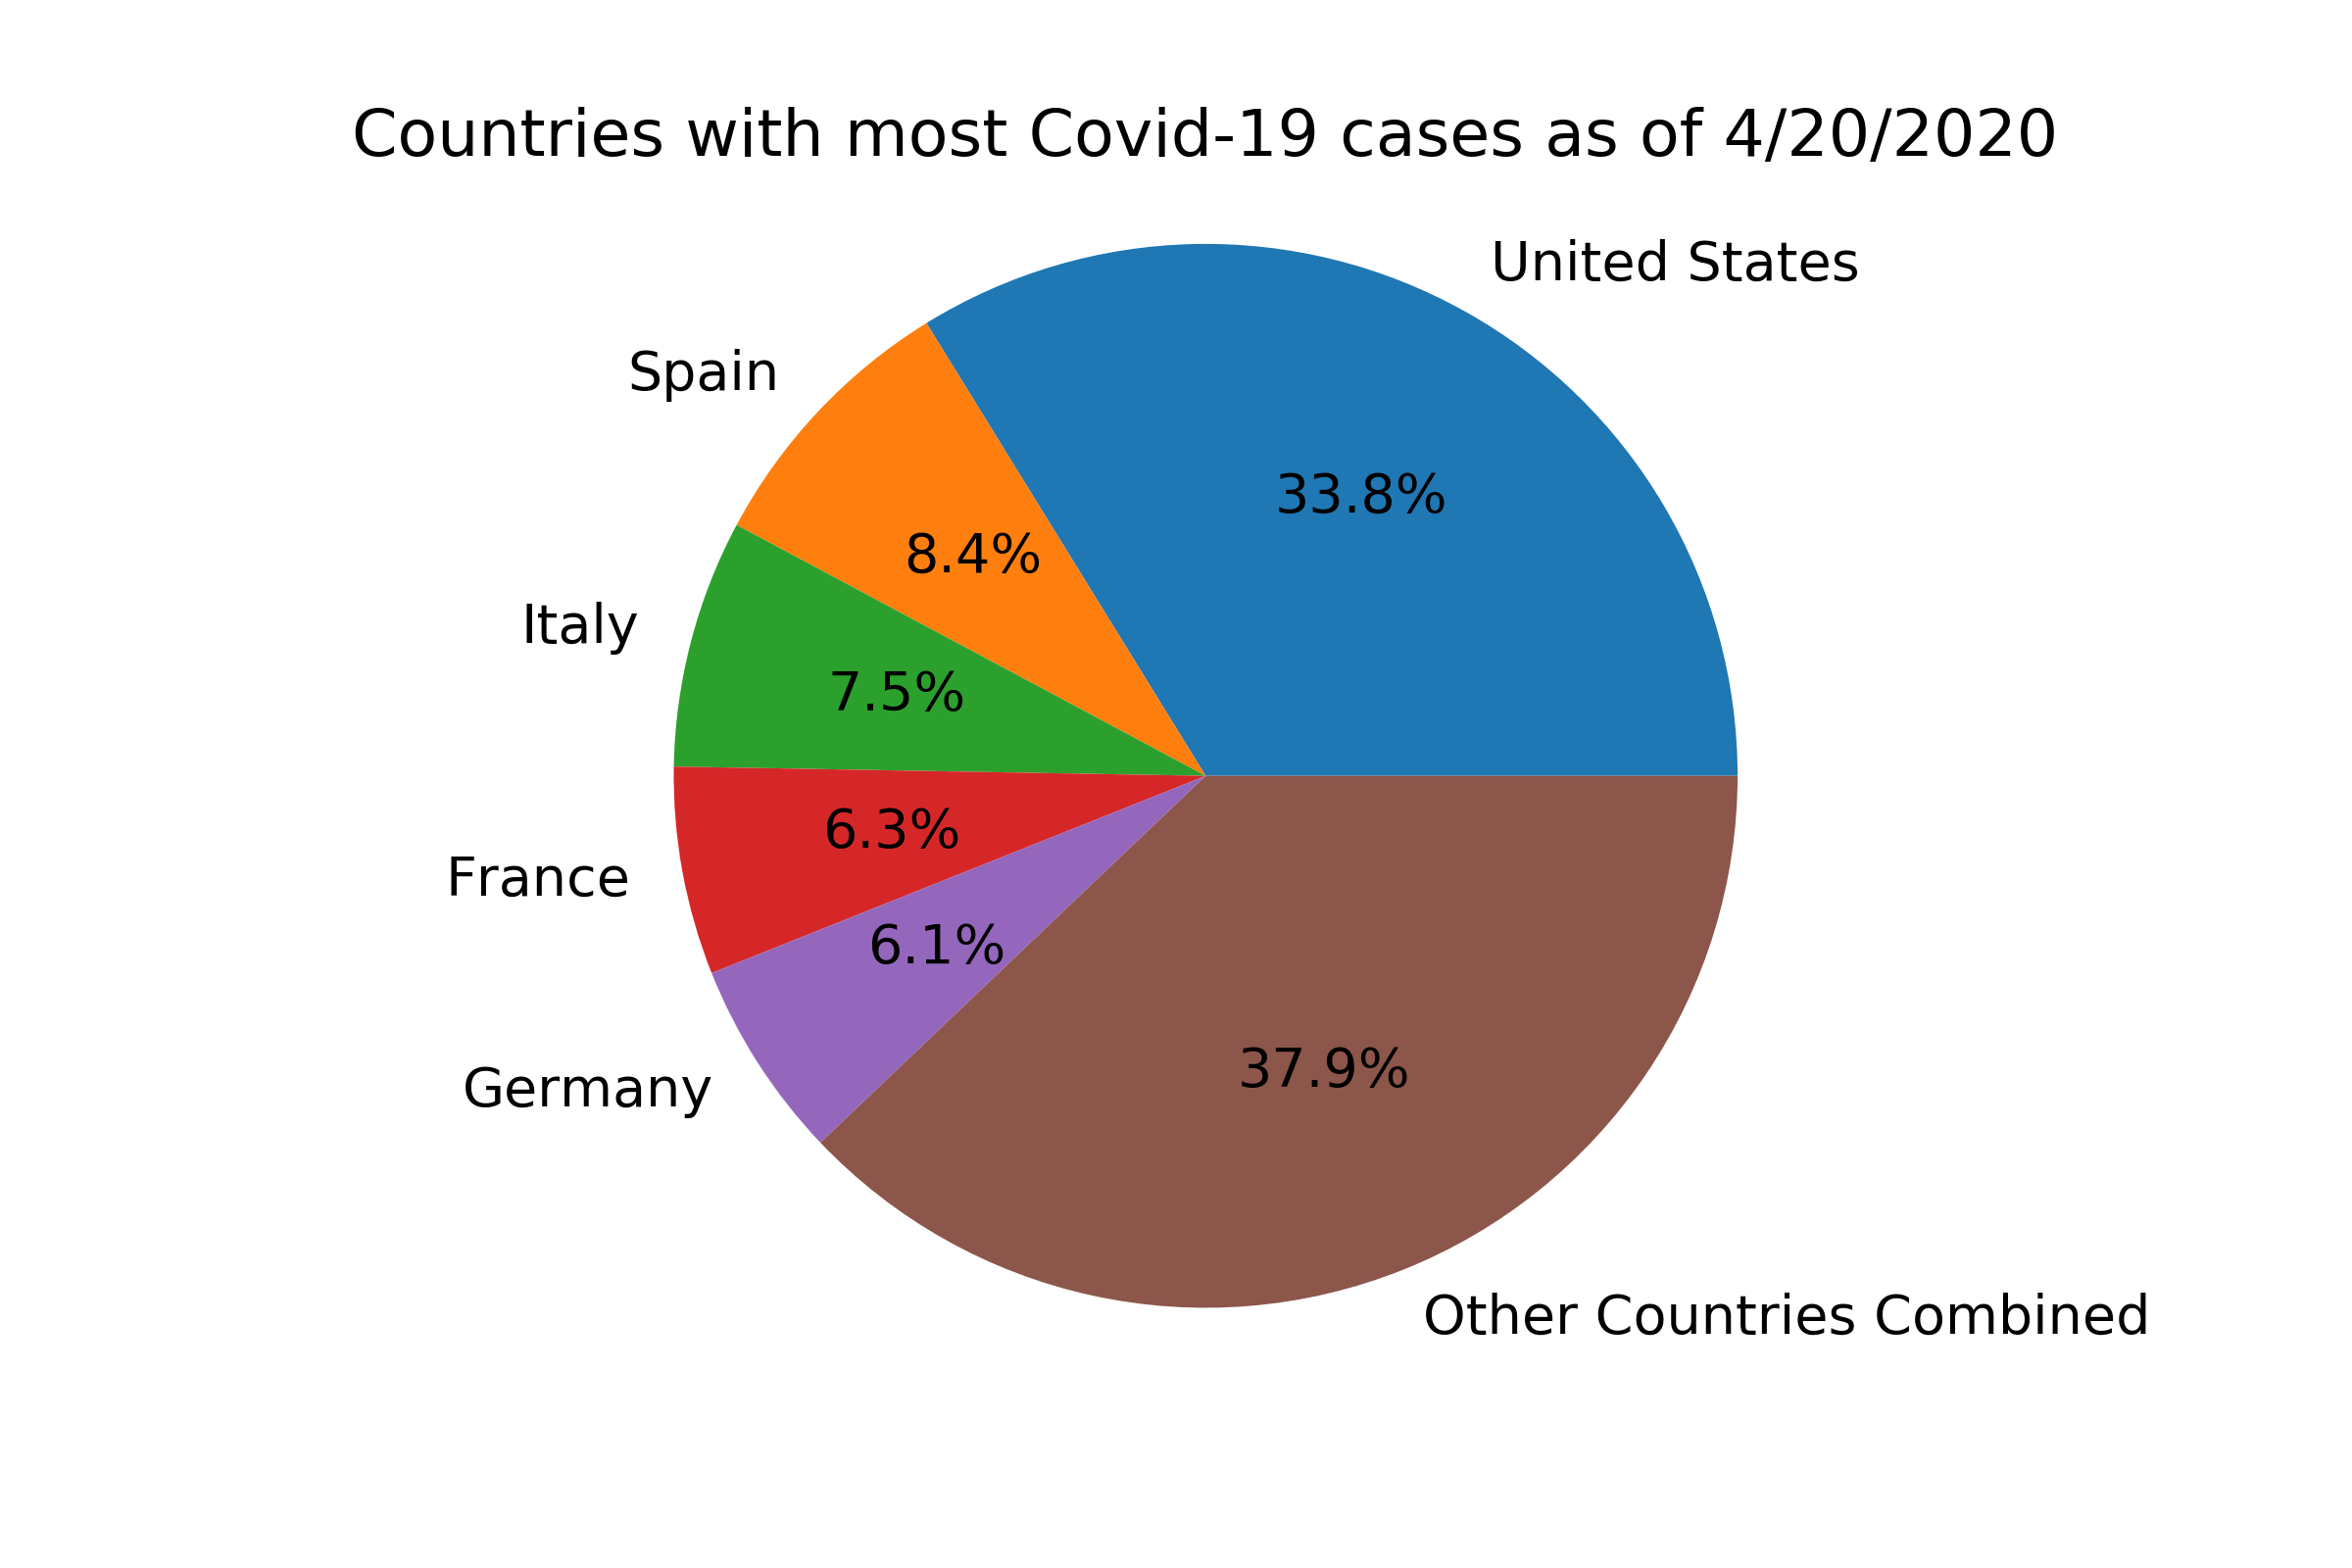
\includegraphics[scale=0.4]{covid-us.png}\\ 
	\centering
	\label{LP-COVID-World}
\end{figure}

	The pie chart visualizes countries with the most Coronavirus cases. The countries in the pie chart are the United States, Spain, Italy, France, Germany, and other countries combined. Other countries combined have the highest number of Coronavirus cases with 37.9 \%. The United States has the second highest number of Coronavirus cases, with 33.8 \%. We decided to have a more in depth analysis on the United States specifically since it has the most cases of Coronavirus compared to other countries like Germany, France, Italy, and Spain. Germany has the lowest number of Coronavirus cases with 6.1 \%.

% Methods Ends

%#############################################################################################################################
% Data Visualization Begins
\section{Data Visualization}\label{sec:data visualization}

	The first data set we looked at is the ozone data set. \cite{eeemonts-2020} The ozone data set consists of collecting the data of ozone levels of countries affected by the Coronavirus. The ozone data set has 100 rows and 83 columns. Columns include Province/State, Country/Region, Latitude/Longitude, and the ozone levels from the date range from January 1, 2020 to March 19, 2020. Ozone levels are measured in dobson units.

	 Our data sets display the ozone levels of countries affected by COVID-19 worldwide. Ozone levels range from the colors blue to green, with blue representing the lowest amount of dobson units and green representing the highest amount of dobson units. Countries that are marked with the color green have the lowest ozone levels and countries that are marked with the color blue have the highest ozone levels. In the case of February 26, 2020, Canada and small countries in Europe have the highest ozone levels. Countries in Latin America and South Asia have the lowest ozone levels. In the case of March 14, 2020, which can be seen in figure 2, countries in Europe have the highest ozone levels. Countries in Latin America and South Asia have the lowest ozone levels.

\begin{figure}[!htbp] % Figure 2 Ozone Measure at Different Latitudes/Longitudes on 2/26/20
	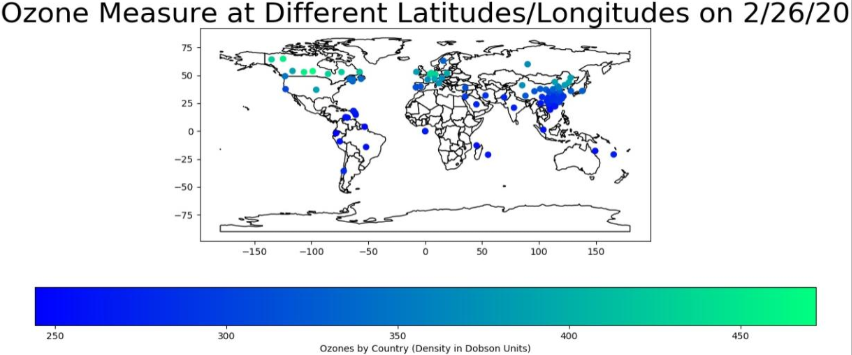
\includegraphics[scale=0.3]{ozone-feb-26.png}\\ 
	\centering
	\label{LP-COVID-Ozone February 26th}
\end{figure}

\begin{figure}[!htbp] % Figure 3 Ozone Measure at Different Latitudes/Longitudes on 3/14/20
	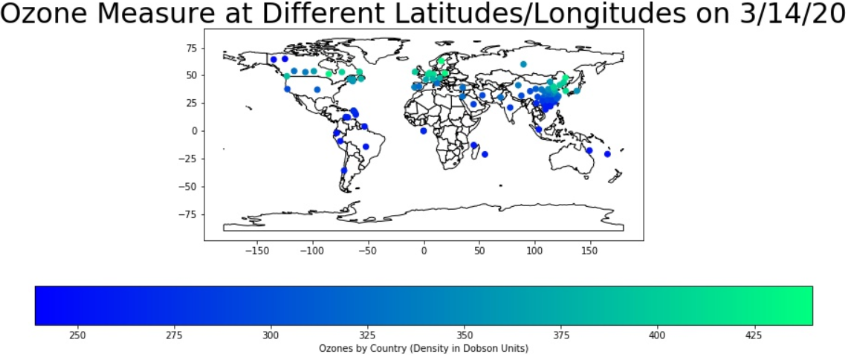
\includegraphics[scale=0.3]{ozone-mar-14.png}\\ 
	\centering
	\label{LP-COVID-Ozone March 14th}
\end{figure}

	The second data set is the humidity level data set. \cite{eeemonts-2020} The humidity level data set has 107 rows and 83 columns. The humidity level data set has attributes: Latitude, Longitude, and the humidity levels from the range from January 1, 2020 to March 19, 2020. The humidity level data set consists of the attributes: Province/State, Country/Region, Latitude/Longitude, and the humidity levels from the dates January 1, 2020 to March 19, 2020. Humidity levels are measured out of one hundred in percentage in units of grams per water vapor per kilogram of air (gram/kilogram).

	Our data sets display the humidity levels of countries affected by Coronavirus worldwide. Humidity levels range from the colors light yellow to dark red, with light yellow representing the lowest humidity level (percent being out of 100) and dark red representing the highest humidity level (percent being out of 100). Countries with the yellow humidity levels have the lowest humidity levels, and countries with dark red humidity levels have the highest humidity levels during the Coronavirus pandemic. On February 26, 2020, the United States and various other small countries in Europe, Latin America and South Asia have the highest humidity levels. Countries in Africa have the lowest humidity levels. In the case of March 14, 2020, whicah can be seen in figure 4, countries in Europe and Latin America have the highest humidity levels. Countries in South Asia have the lowest humidity levels.

\begin{figure}[!htbp] % Figure 4 Humidity at Different Latitudes/Longitudes on 2/26/20
	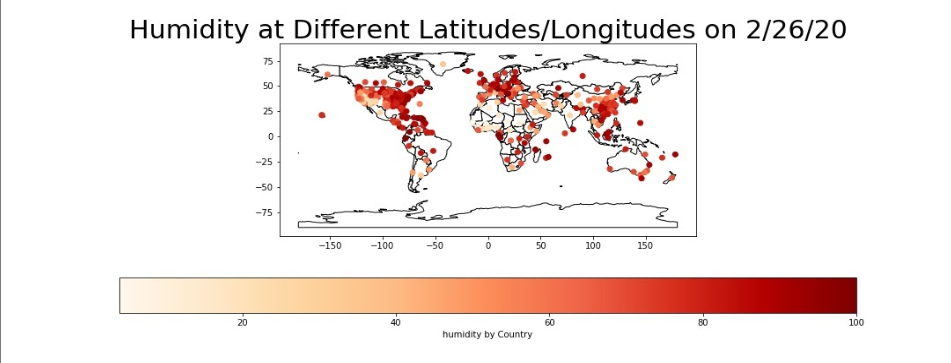
\includegraphics[scale=0.3]{humidity-feb-26.png}\\
	\centering
	\label{LP-COVID-Humidity February 26th}
\end{figure}

\begin{figure}[!htbp] % Figure 5 Humidity at Different Latitudes/Longitudes on 3/14/20
	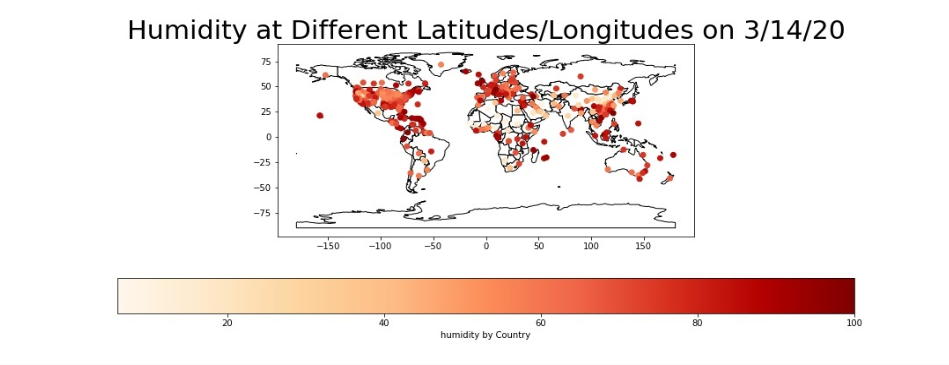
\includegraphics[scale=0.3]{humidity-mar-14.png}\\
	\centering
	\label{LP-COVID-Humidity March 14th}
\end{figure}

	Our third data set is the Corona Mortality Rate data set. \cite{Mooney-2020} The Corona Mortality Data set has 107 rows and 8 columns.The Corona Mortality Rate data set includes the attributes: Unnamed: 0, Country, Confirmed, Deaths, Mortality Rate, Latitude, Longitude, and Country Code.

	Our data sets display the mortality rate of countries affected by Coronavirus worldwide.As shown later in our preliminary results, mortality rate due to Coronavirus ranges from the colors light yellow to dark red, with light yellow representing the lowest mortality rate and dark red representing the highest mortality rate. Countries that are marked with the color yellow have the lowest mortality rate and countries marked with the color dark red have the highest mortality rate during the Coronavirus pandemic. On March 11, 2020, some countries in the southern region of Africa have the highest mortality rate. The United States, Asia, and Europe have the lowest mortality rates.

	In this section of the report we decided to narrow our view into more specific areas, specifically California. After deciding on California as our main focus of study, we decided to narrow it down further to individual counties since counties are small enough to have a consistent weather pattern across its region. We began our exploratory analysis and descriptive analysis of three different counties.\cite{NOAA-2020} \cite{MyrnaMFL-2020} These three counties we selected were Los Angeles, Orange, and Santa Clara counties. We decided on these three counties because the Los Angeles and Orange counties were two very similar counties due to them being geographical neighbors. Also the Santa Clara county was further and typically known for different weather patterns from the Los Angeles and Orange counties. With these three counties, our team started our exploratory analysis and descriptive analysis.

\begin{figure}[!htbp] % Figure 6 Trend Line of COVID-19 cases in Orange County within 30 days
	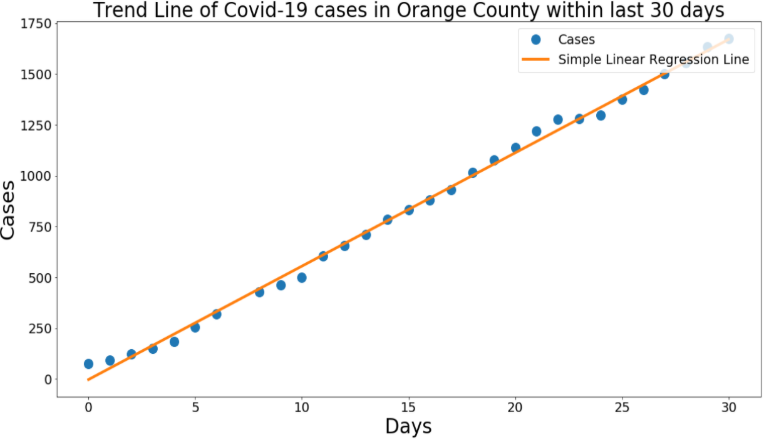
\includegraphics[scale=0.45]{covid-orange.png}\\ 
	\centering
	\label{LP-COVID-Orange County}
\end{figure}

	As you can see in the above visualization, from March 21st to April 20th, we noticed a steady increasing trendline in increasing coronavirus cases. We used simple linear regression in order to show that COVID-19 is increasing at an alarming rate. Next we visualized maximum temperature and minimum temperature in order to visualize and discover any visual trends or clusters as information. 

% Data Visualization Ends
%#############################################################################################################################
% Preliminary Results Begins
\section{Preliminary Results}\label{sec:preliminary results}

	In the graph "Ozone Measure at Different Latitude/Longitutdes on 2/26/20", around latitude 40°, many locations have ozone levels ranging from 275 to 350 dobson units, which means that there was heavy exposure to UV rays . So if areas had shifted in the ozone layer, then the Coronavirus spread could differ as the disease would have a harder time surviving out in the environment. Most viruses cannot survive high temperatures. 

	In the graph "Ozone Measure at Different Latitudes/Longitudes on 3/14/20", the low standard deviation of ozone measure proves that ozone will not change much over time and thus will most likely not contribute much to the spread or slow down of Coronavirus according to the data. We also noticed the standard deviation of minimum temperature to remain consistent for many countries . Temperature is measured in degrees Fahrenheit.

\begin{figure}[!htbp] % Figure 7 Ozone Over Various Latitudes on 2/6/20	
	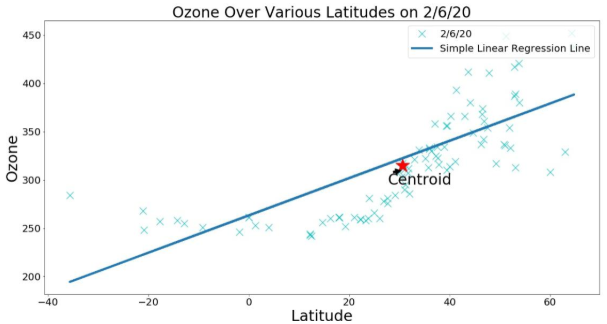
\includegraphics[scale=0.6]{ozone-feb-centroid.png}\\ 
	\centering
	\label{LP-COVID-Ozone February 26th}
\end{figure}

\begin{figure}[!htbp] % Figure 8 Ozone Over Various Latitude on 3/14/20
	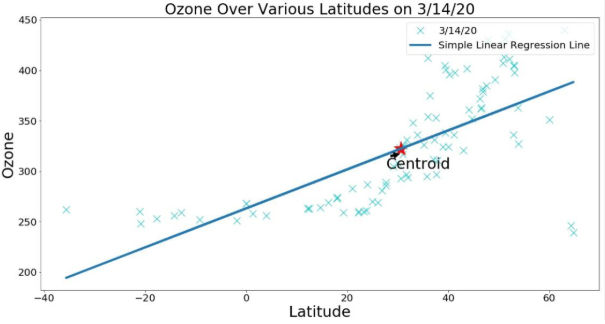
\includegraphics[scale=0.6]{ozone-mar-centroid.png}\\ 
	\centering
	\label{LP-COVID-Ozone March 14th}
\end{figure}

	As you can see in the graph for humidity levels at different latitudes/longitudes, approximately around latitude 40° which is measured around the globe, many locations have a humidity ranging from about 60 to 90 grams per water vapor per kilogram of air (gram/kilogram), meaning that the locations are relatively moisturized. Humidity levels are measured in grams per water vapor per kilogram of air (gram/kilogram). Ozone levels are measured in dobson units. This shows that latitude 40° also has more cases of coronavirus than other latitudes.

\begin{figure}[!htbp] % Figure 3 Humidity at Different Latitudes on 2/26/20
	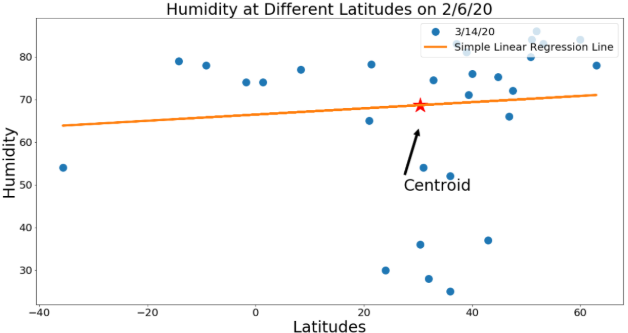
\includegraphics[scale=0.6]{humidity-feb-centroid.png}\\
	\centering
	\label{LP-COVID-Humidity February 26th}
\end{figure}

\begin{figure}[!htbp] % Figure 4 Humidity at Different Latitudes on 3/14/20
	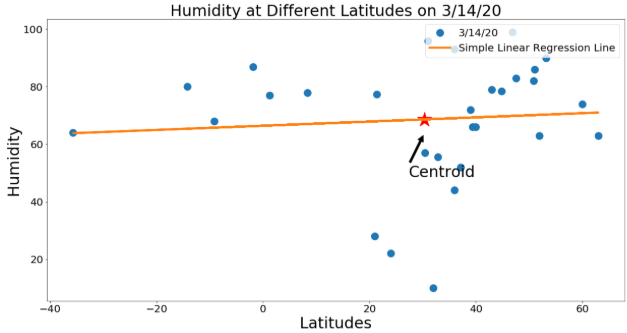
\includegraphics[scale=0.6]{humidity-mar-centroid.png}\\
	\centering
	\label{LP-COVID-Humidity March 14th}
\end{figure}

\clearpage

	As a result, it will not be as useful as maximum temperature. Latitudes with moderate high weather have the most cases of Coronavirus. No matter what latitude, Coronavirus can still exist and spread depending on the mortality rate, which is measured by how long a person lives. The highest mortality rate recorded was at 20 \% at latitudes ranging from 20° to 40°. Outside of the latitude ranges from 20° to 40°, mortality rate started to decrease sharply to zero. This mortality-latitude relationship is likely due to humidity at those latitudes. The humidity levels and ozone measure graphs both show a positive correlation between humidity, ozone, and latitude of countries respectively. After latitude 40°, humidity levels increase from 40 \% to 60\% and ozone levels increase up to 350 dobson units on 3/14/20 (Pi Day).

\begin{figure}[!htbp] % Mortality Rate of Different Countries represented in a heatmap as of March 11th
	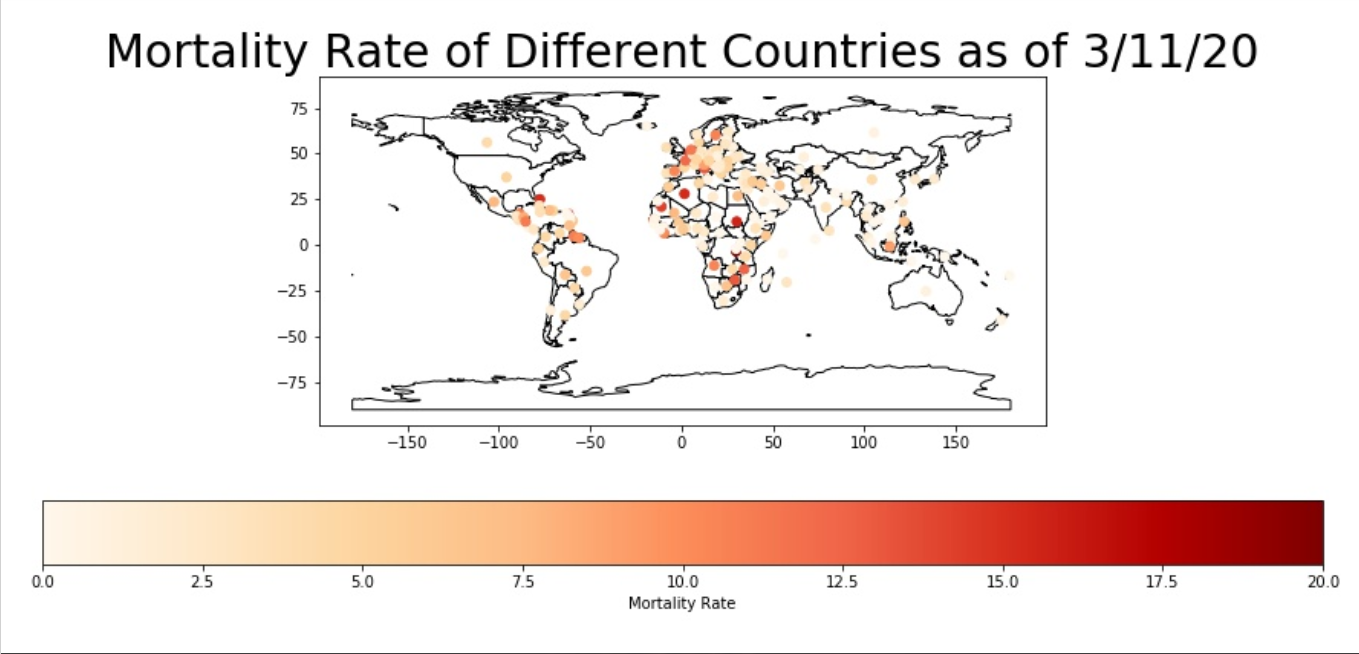
\includegraphics[scale=0.19]{mortality-mar-11.png}\\
	\centering
	\label{LP-COVID-Mortality Rate March 11th}
\end{figure}

	We discovered that there was a standard deviation of 3.4° F and a mean of 50.22° F. This information for standard deviation and mean show that the minimum temperature was very consistent as the data for standard deviation was very low with two standard deviations of change in the temperature result of ±6.8 F, which encompasses 95 \% of the minimum temperature range. This range of 12° F is very small, and will mostly likely not increase nor decrease the COVID-19 spread since it's stagnant. Max tempature on the other hand, has a standard devation of 6.1, thus 2 standard devations is ±12.2° which will create a 24.4 degree range where the max tempature can fluctuate. This large fluxation area, could allow for the disease to spread more in the lower range of the 24 degree, while decreasing the spread at the top end of the spectrum. Using this reasoning we can assume, that areas that have high fluctuation of tempature will have varying rate of covid-19 surviving in the environment. Some cool days it can spread more, and on warmer day the disease will spread less. However during the night when minimum tempature occurs most often, the disease will survive at the same rate. Using this logic we can apply this to many other counties and see which counties have a chance to have a change of tempature, and thus influence the survival of the COVID-19 in their environment. 

{\SetAlgoNoLine
	\begin{algorithm}
		\caption{Standard Deviation}
		\label{Algo: Calculate Standard Deviation:BWLP}
		Input: $\ 
		\ N = \ the \ size \ of \ the \ population, \newline
		\ x_i = \ each \ value \ from \ the \ population, \newline
		\ \mu = \ the \ population \ mean
		$\\
		Output: $  \alpha = \ population \ and \ standard \ deviation $\\
			
$ 			 	 \alpha = \sqrt\frac{\sum (x_i - \mu)^2}{N} $
	\end{algorithm}

	 We also formed hypotheses, based off our California counties visualizations and then used descriptive analysis to support our hypotheses. For our first hypothesis, we believed Orange County had a very stable and consistent minimum temperature since the minimum temperature seemed visually clustered in a range of about 10° F. Using this hypothesis related to the minimum temperature of Orange County, we used descriptive analysis, specifically mean and standard deviation, to determine if our hypothesis had any validity.
	
	The minimum temperature in Orange County has a consistency within a 10 degree range of 45 to 55° F with a mean of 50.52° F and a standard deviation of 3.40° F. This shows that the minimum temperature on average stays consistent. The maximum temperature in Orange County fluctuated more than minimum temperature. The mean is 68.12° F and  has a standard deviation of 6.10° F. This shows that maximum temperature is volatile.

 \begin{figure}[!htbp] % Figure 3 Minimum Temperature of Orange County
	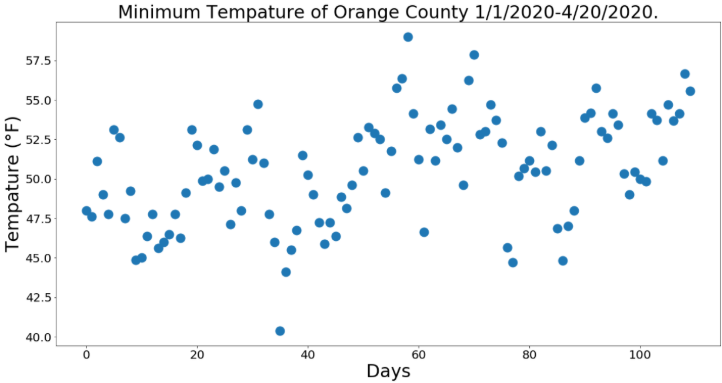
\includegraphics[scale=0.45]{min-orange.png}\\ 
	\centering
	\label{LP-COVID-Minimum Temperature}
\end{figure}

\begin{figure}[!htbp] % Figure 4 Maximum Temperature of Orange County
	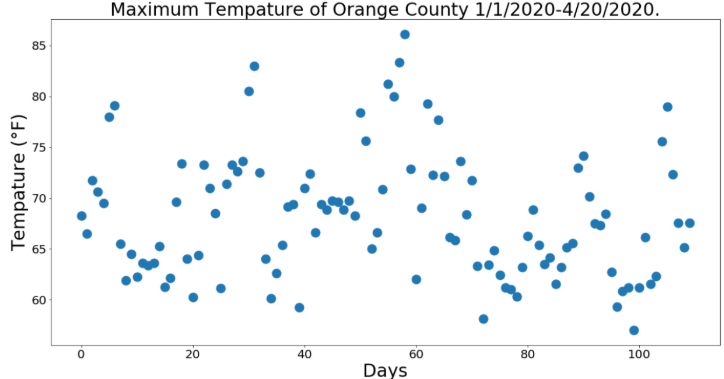
\includegraphics[scale=0.45]{max-orange.png}\\ 
	\centering
	\label{LP-COVID-Maximum Temperature}
\end{figure}

% Preliminary Results Ends
%#############################################################################################################################
\section{Conclusion}
\label{sec: conclusion}

	With COVID-19 and SARS having similarities in its country of origin, climate, scale and transmission it is highly probable that these viruses are closely related. Through this we can look at past studies conducted on SARS and correlate that to the ongoing COVID-19 pandemic. But it is worth noting that the SARS pandemic of 2003 and COVID-19 show a great disparity in terms of data, research, and lack of modernized technologies. Nonetheless, SARS share similarities in terms of its transmission with the Coronavirus’s methods of transmission, through the respiratory systems and the effects weather has on these two viruses. In our research, we look at how multiple aspects of weather such as humidity, ozone, and temperature may influence the Coronavirus.

	We can see that around 40th parallel north (40° latitude) shows heavy exposure to UV rays. Based on this fact, the Coronavirus spread may differ as the disease has a much harder time surviving in high temperature environments. But we must also consider our low standard deviation results. Which proves that ozone may contribute overall to the spread of the Coronavirus. Also, our standard deviation for the minimum temperature remained consistent for many countries

	It is also worth noting that at this latitude there are multiple locations with humidity’s ranging from 60 to 90 g per water vaper per kg of air. These areas are high in moisture. It is worth noting that people are more prone to illnesses in high humidity. Latitudes with moderate to high weather have the most Coronavirus cases. But no matter what latitude, Coronavirus will still exist and spread in relation to the mortality rate. We can see a 20 \% mortality rate in those latitudes ranging from 20° to 40°. Outside of those ranges we can see that the mortality rate begins to decrease to zero. This relationship is due to humidity at these levels.

	We have concluded our study on up to 28 counties, which have a minimum of 100 cases in each county. We plan on continuing this study by making use of clustering to see which counties have a similar tempature range at different times of the year using our weather data. Though this we will predict which counties will have a chance of lower/higher COVID-19 surivival rate in their environment. We also plan to list counties that maintain a stable weather pattern which will not affect the COVID-19 survival rate in the environment

	To reiterate it is safe to assume that the weather has some degree of influence on Coronavirus. We can see that the number of confirmed coronavirus cases varies differently based on humidity and that countries located on the 40th parallel north, which spans across the United States and China may see an decrease in coronavirus cases as the weather becomes warmer. Since the ozone’s standard deviation is low, there is not enough direct evidence in affecting weather other than showing consistent data for our visualizations.

	Through this project we hope to bring more awareness and insight into the ongoing pandemic that is the Coronavirus. It is highly recommended to provide any contribution to slow the spread of the Coronavirus. The information is widely available online for the use of others to use as well. We are just one of the many groups of people who strive to help in the flattening the curve and stop the coronavirus pandemic.

%#############################################################################################################################
% Contributions
\ifCLASSOPTIONcompsoc
\section*{Contributions}
Madhuri, Harpreet, Michael 
\begin{itemize}
	\item Data Cleaning  
	
	\item Data Structuring

	\item Transformation of Graphs

	\item Descriptive Analysis

	\item Predictive Analysis

	\item Prescriptive Analysis
\end{itemize}
Joshua, Micah, Xavier, Michael
\begin{itemize}
	\item Data Visualization
	
	\item Report Creation
	
	\item Presentation

	\item Analysis Visualization 
\end{itemize}
%#############################################################################################################################
\ifCLASSOPTIONcompsoc
\section*{Acknowledgments}
	Our team would like to acknowledge our professor, Dr. Pirouz for providing us this wonderful opportunity to work on a project such as this. We would also like acknowlege the amount of time and effort she provides us so that we can apply the skills we have learned into a real world application. We would also like to thank open source data providers for providing open data sets for students like us to help provide research and insight into the over bearing pandemic that is the Corona Virus.
%#############################################################################################################################
\else
\section*{Acknowledgment}
\fi

\ifCLASSOPTIONcaptionsoff
  \newpage
\fi
%#############################################################################################################################
% References
  \bibliographystyle{naturemag}
  \bibliography{bibilo}
%############################################################################################################################# 
\end{document}


